\documentclass{beamer}
\usepackage{bookmark}

\usetheme{Copenhagen}

\title{Compression de Huffman}
\author{Benguezzou Mohamed \\ Fiszer Andrea}

\institute{Licence 2 semestre 4}
\titlegraphic{
\includegraphics[width=0.3\textwidth]{../assets/fst-logo.png}}
\date{} 

\begin{document}

\begin{frame}
    \titlepage
\end{frame}

\begin{frame}{Table des matières}
    \tableofcontents
\end{frame}

\section{Protocole expérimental}
\subsection{Analyse des facteurs influants}

\begin{frame}{Analyse des facteurs influants}

    \begin{center}
        \large\textbf{Quel facteur influence la structure de l'arbre de Huffman ?}
    \end{center}

    \begin{columns}[T]

        \begin{column}{0.5\textwidth}
            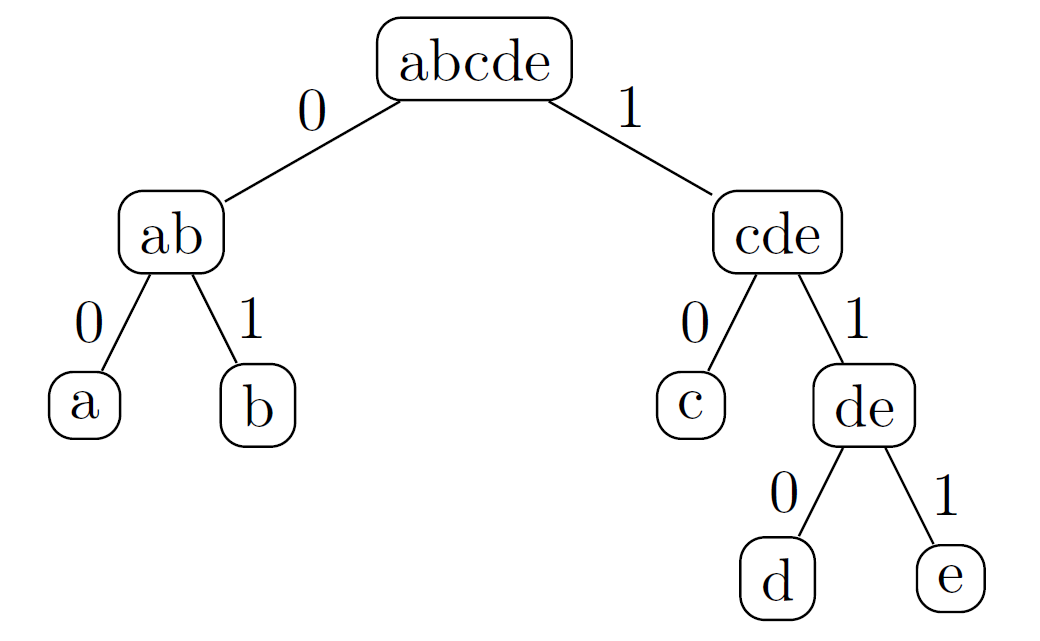
\includegraphics[width=\textwidth]{../assets/huffman-tree-example.png}
        \end{column}

        \begin{column}{0.5\textwidth}
            \vspace{20pt}
            \centering

            \begin{itemize}
                \item La fréquence d'apparition des caractères
                \item Le nombre de feuilles, i.e la taille de l'alphabet
            \end{itemize}

        \end{column}
    \end{columns}
\end{frame}

\subsection{Génération des fichiers de test}

\begin{frame}{Génération des fichiers de test}
    \centering
    \large\textbf{Comment générer des fichiers de test ?}

    \vspace{20pt}

    \begin{itemize}
        \item \texttt{--num\_chars} : la taille de l'alphabet.
        \item \texttt{--size} : la taille du fichier généré.
        \item \texttt{--output\_dir} : le répertoire de sortie.
    \end{itemize}

    \vspace{20pt}
    Cela nous permet de générer des fichiers en controlant la
    \textbf{taille de l'alphabet} et la \textbf{taille du fichier}.

\end{frame}

\subsection{Lois de génération}
\begin{frame}{Lois de génération}
    \centering
    \large\textbf{Comment contrôler la fréquence d'apparition des caractères ?}

    \vspace{15pt}
    \begin{itemize}
        \item Loi uniforme
        \item Loi normale
        \item Loi de puissance ($P(x) = \frac{1}{x^\alpha} ;$ avec $\alpha = 1.5$)
        \item Loi aléatoire
        \item Loi linéaire
    \end{itemize}

    \vspace{10pt}
    L'utilisation de ces lois nous permet de contrôler \textbf{la fréquence}
    d'apparition des caractères dans les fichiers générés.

\end{frame}


\subsection{Expérimentation}


\begin{frame}{Expérimentation - Lois de génération}
    \begin{columns}[T]
        \begin{column}{0.6\textwidth}
            \begin{figure}
                \centering
                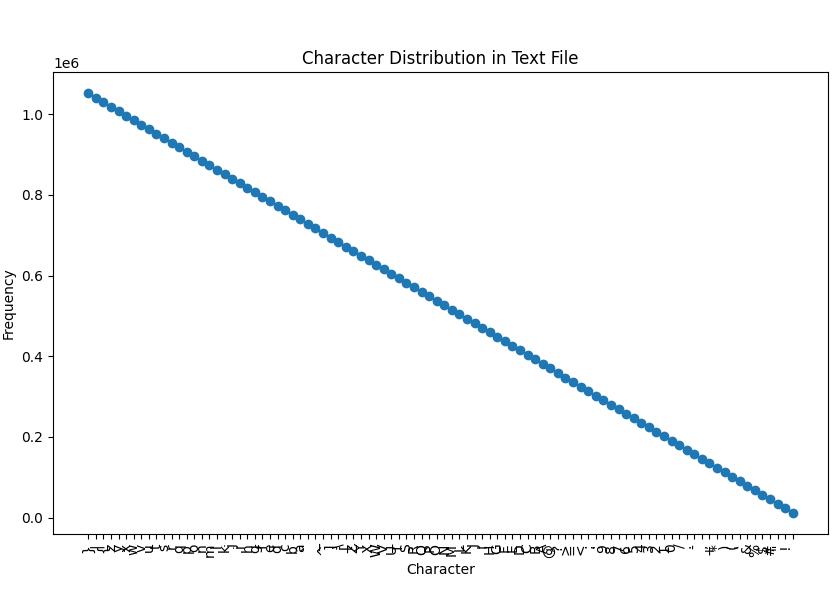
\includegraphics[width=\textwidth]{../assets/linear.png}
                \caption{Loi linéaire}
            \end{figure}
        \end{column}
        \begin{column}{0.5\textwidth}
            \vspace{10pt}
            \textbf{Hypothèse} \\
            \vspace{25pt}
            \begin{itemize}
                \item Faible différence des profondeurs des feuilles.
                \item Gain de compression pas très élevé.
            \end{itemize}
        \end{column}
    \end{columns}
\end{frame}

\begin{frame}{Expérimentation - Lois de génération}
    \begin{columns}[T]
        \begin{column}{0.6\textwidth}
            \begin{figure}
                \centering
                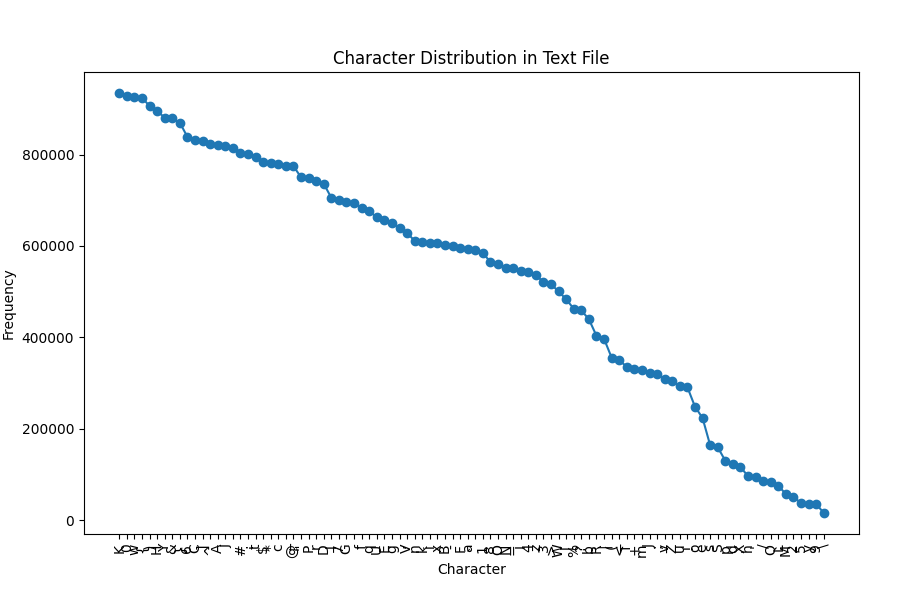
\includegraphics[width=\textwidth]{../assets/random.png}
                \caption{Loi aléatoire}
            \end{figure}
        \end{column}
        \begin{column}{0.5\textwidth}
            \vspace{10pt}
            \textbf{Hypothèse} \\
            \vspace{20pt}
            \begin{itemize}
                \item Suit approximativement une loi linéaire.
                \item Gain de compression similaire à la loi linéaire.
            \end{itemize}
        \end{column}
    \end{columns}
\end{frame}

\begin{frame}{Expérimentation - Lois de génération}
    \begin{columns}[T]
        \begin{column}{0.6\textwidth}
            \begin{figure}
                \centering
                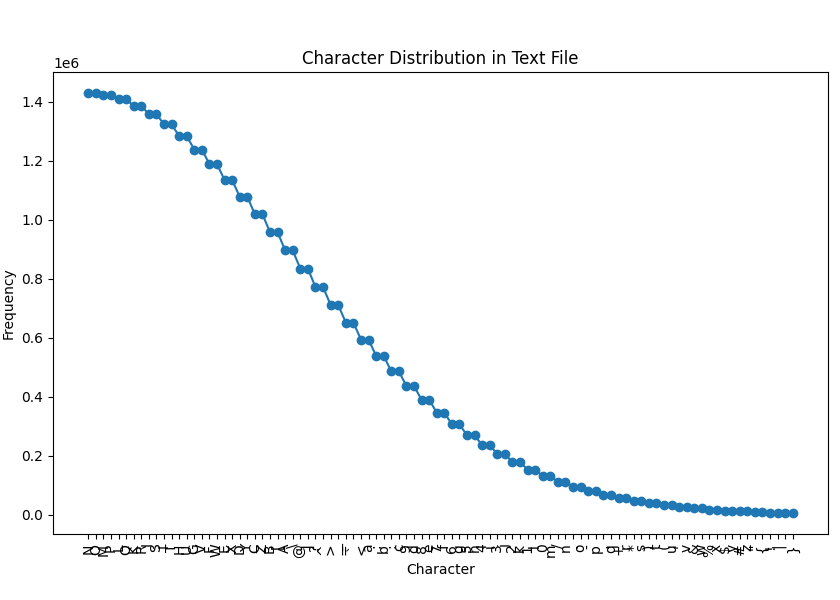
\includegraphics[width=\textwidth]{../assets/normal.png}
                \caption{Loi normale}
            \end{figure}
        \end{column}
        \begin{column}{0.5\textwidth}
            \vspace{10pt}
            \textbf{Hypothèse} \\
            \vspace{10pt}
            \begin{itemize}
                \item Meilleure compression que la loi linéaire.
                \item Profondeur des feuilles plus inégale.
            \end{itemize}
        \end{column}
    \end{columns}
\end{frame}

\begin{frame}{Expérimentation - Lois de génération}
    \begin{columns}[T]
        \begin{column}{0.6\textwidth}
            \begin{figure}
                \centering
                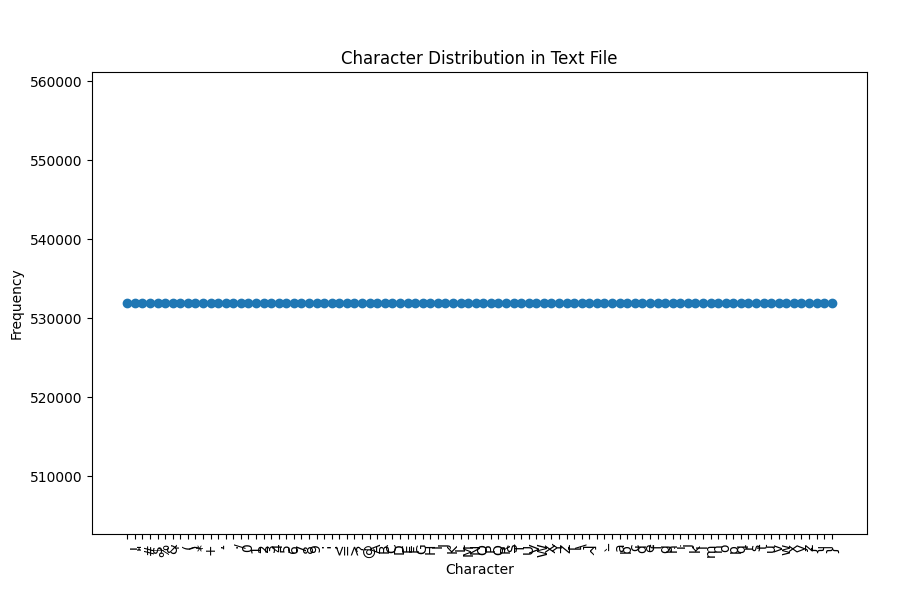
\includegraphics[width=\textwidth]{../assets/uniform.png}
                \caption{Loi uniforme}
            \end{figure}
        \end{column}
        \begin{column}{0.5\textwidth}
            \vspace{10pt}
            \textbf{Hypothèse} \\
            \vspace{10pt}
            \begin{itemize}
                \item Fréquence d'apparition des caractères égale.
                \item Faible gain de compression par rapport aux autres lois.
            \end{itemize}
        \end{column}
    \end{columns}
\end{frame}


\begin{frame}{Expérimentation - Lois de génération}
    \begin{columns}[T]
        \begin{column}{0.6\textwidth}
            \begin{figure}
                \centering
                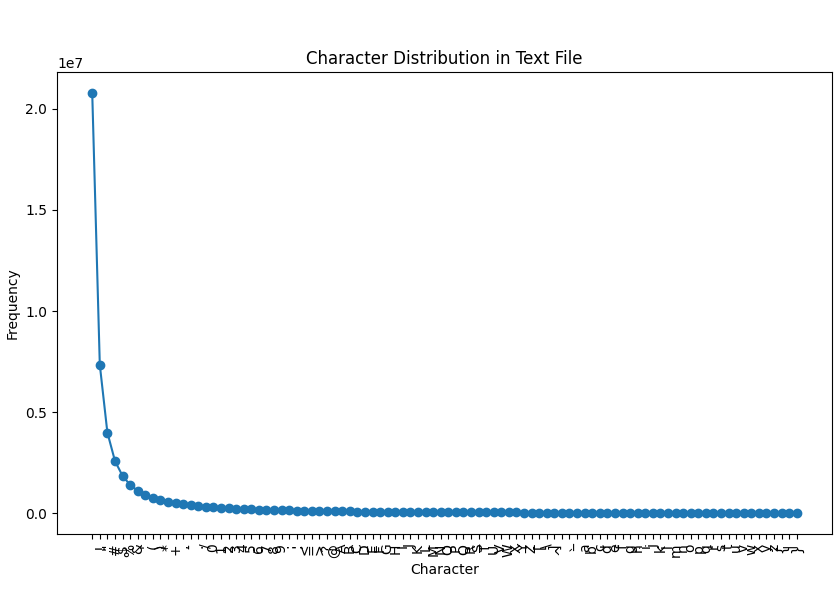
\includegraphics[width=\textwidth]{../assets/puissance.png}
                \caption{Loi de puissance}
            \end{figure}
        \end{column}
        \begin{column}{0.5\textwidth}
            \vspace{10pt}
            \textbf{Hypothèse} \\
            \vspace{10pt}
            \begin{itemize}
                \item Meilleure résultat de compression attendu.
                \item Fréquence d'apparition des caractères très inégale.
                \item Gain de compression élevé.
            \end{itemize}
        \end{column}
    \end{columns}
\end{frame}




\section{Analyse et interprétation}
\begin{frame}{Analyse des résultats}
    \centering
    \large\textbf{Quelques chiffres}

    \vspace{20pt}
    \begin{itemize}
        \item 80 fichiers générés
        \item 5 lois de génération
        \item 10 tailles de fichier (de 1000 octets à 50 000 000 octets)
        \item 7 tailles d'alphabet (de 2 à $94$ puissance de $2$)
    \end{itemize}
\end{frame}

\begin{frame}{Définitions}
    \centering
    \large\textbf{Quelques définitions}
    \vspace{10pt}
    \begin{columns}[T]
        \begin{column}{0.9\textwidth}
            \begin{flushleft}
                \textbf{Taille originale} : taille du fichier avant compression. \\
                \vspace{10pt}

                \textbf{Taille compressée} : taille du fichier après compression. \\
                \vspace{10pt}

                \textbf{Taille de l'alphabet} : nombre de caractères différents. \\
                \vspace{10pt}

                \textbf{Taux de compression} : $\frac{taille\_originale}{taille\_compressee}$ \\
                \vspace{10pt}

                \textbf{Pourcentage de compression} : \\

                \centering
                $ = \frac{taille\_originale - taille\_compressee}{taille\_originale} \times 100$ \\
            \end{flushleft}
        \end{column}
    \end{columns}
\end{frame}


\subsection*{Taille des fichiers compressés selon la taille d'origine}
\begin{frame}{Taille des fichiers compressés selon la taille d'origine}
    \begin{columns}[T]
        \begin{column}{0.9\textwidth}
            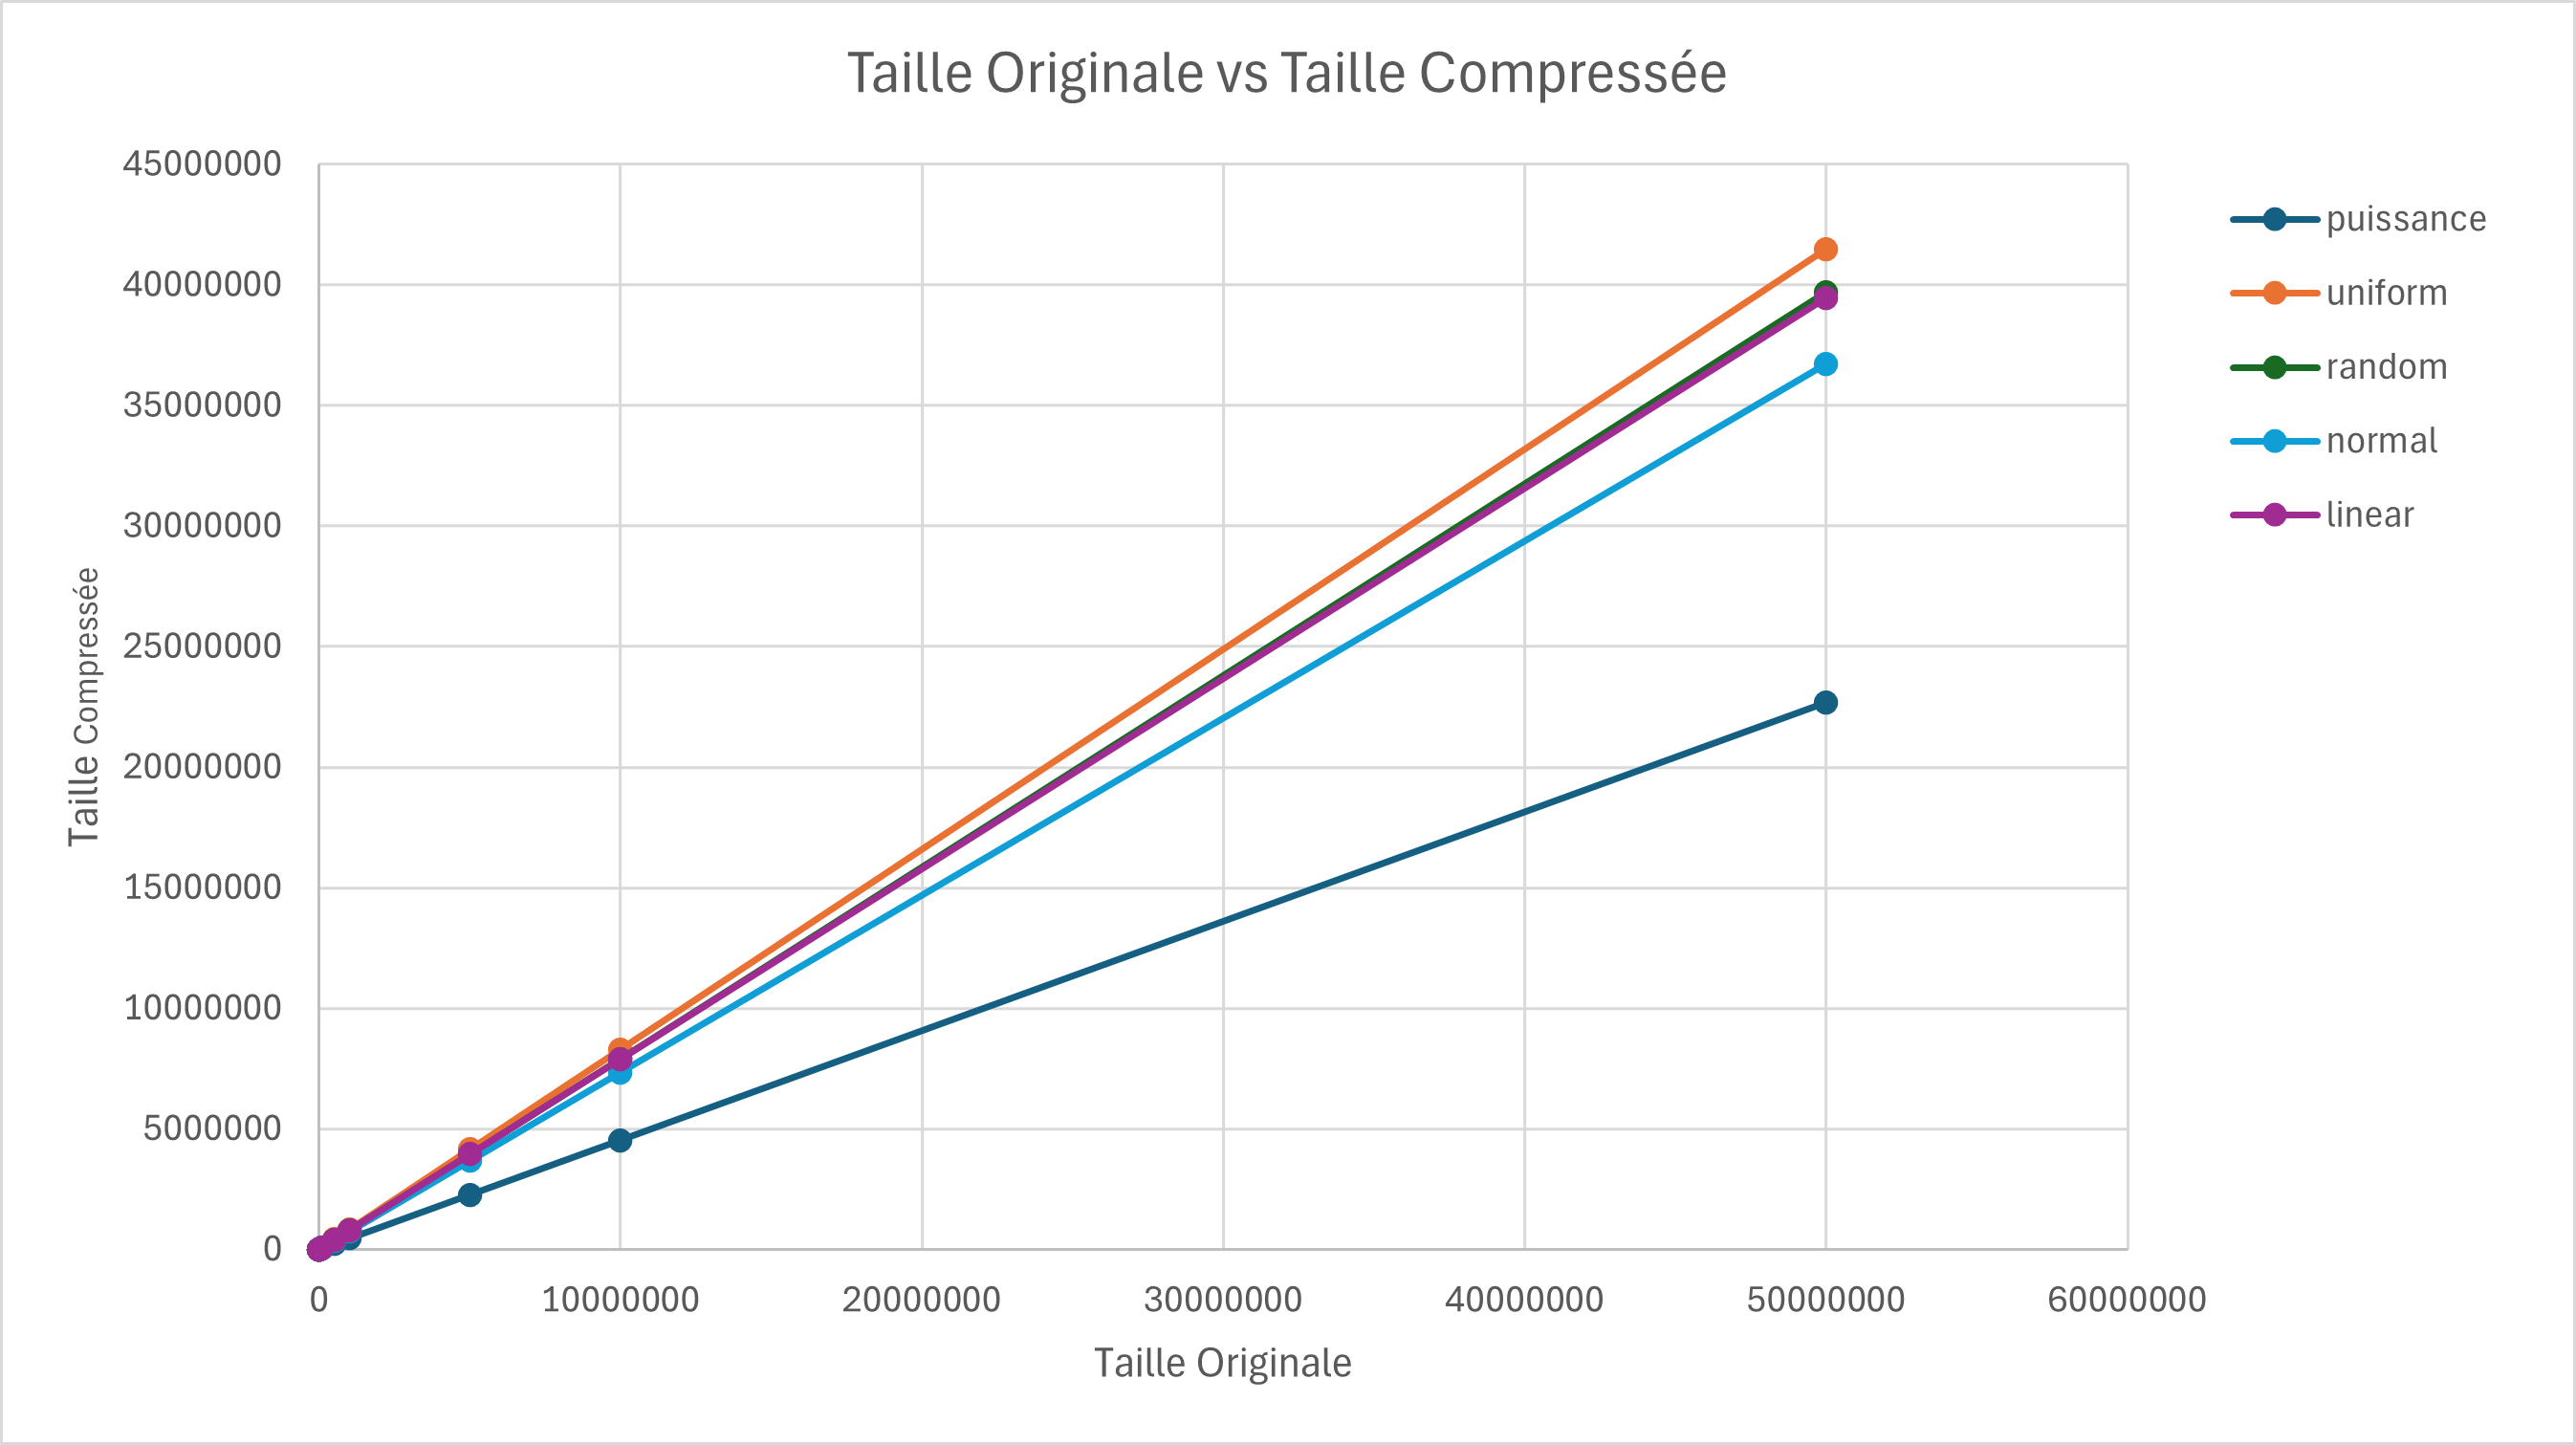
\includegraphics[width=\textwidth]{../assets/taille-originale-vs-compressee.png}
        \end{column}
    \end{columns}
\end{frame}


\subsection*{Pourcentage de compression selon la loi de génération}
\begin{frame}{Pourcentage de compression selon la loi de génération}
    \begin{columns}[T]
        \begin{column}{0.9\textwidth}
            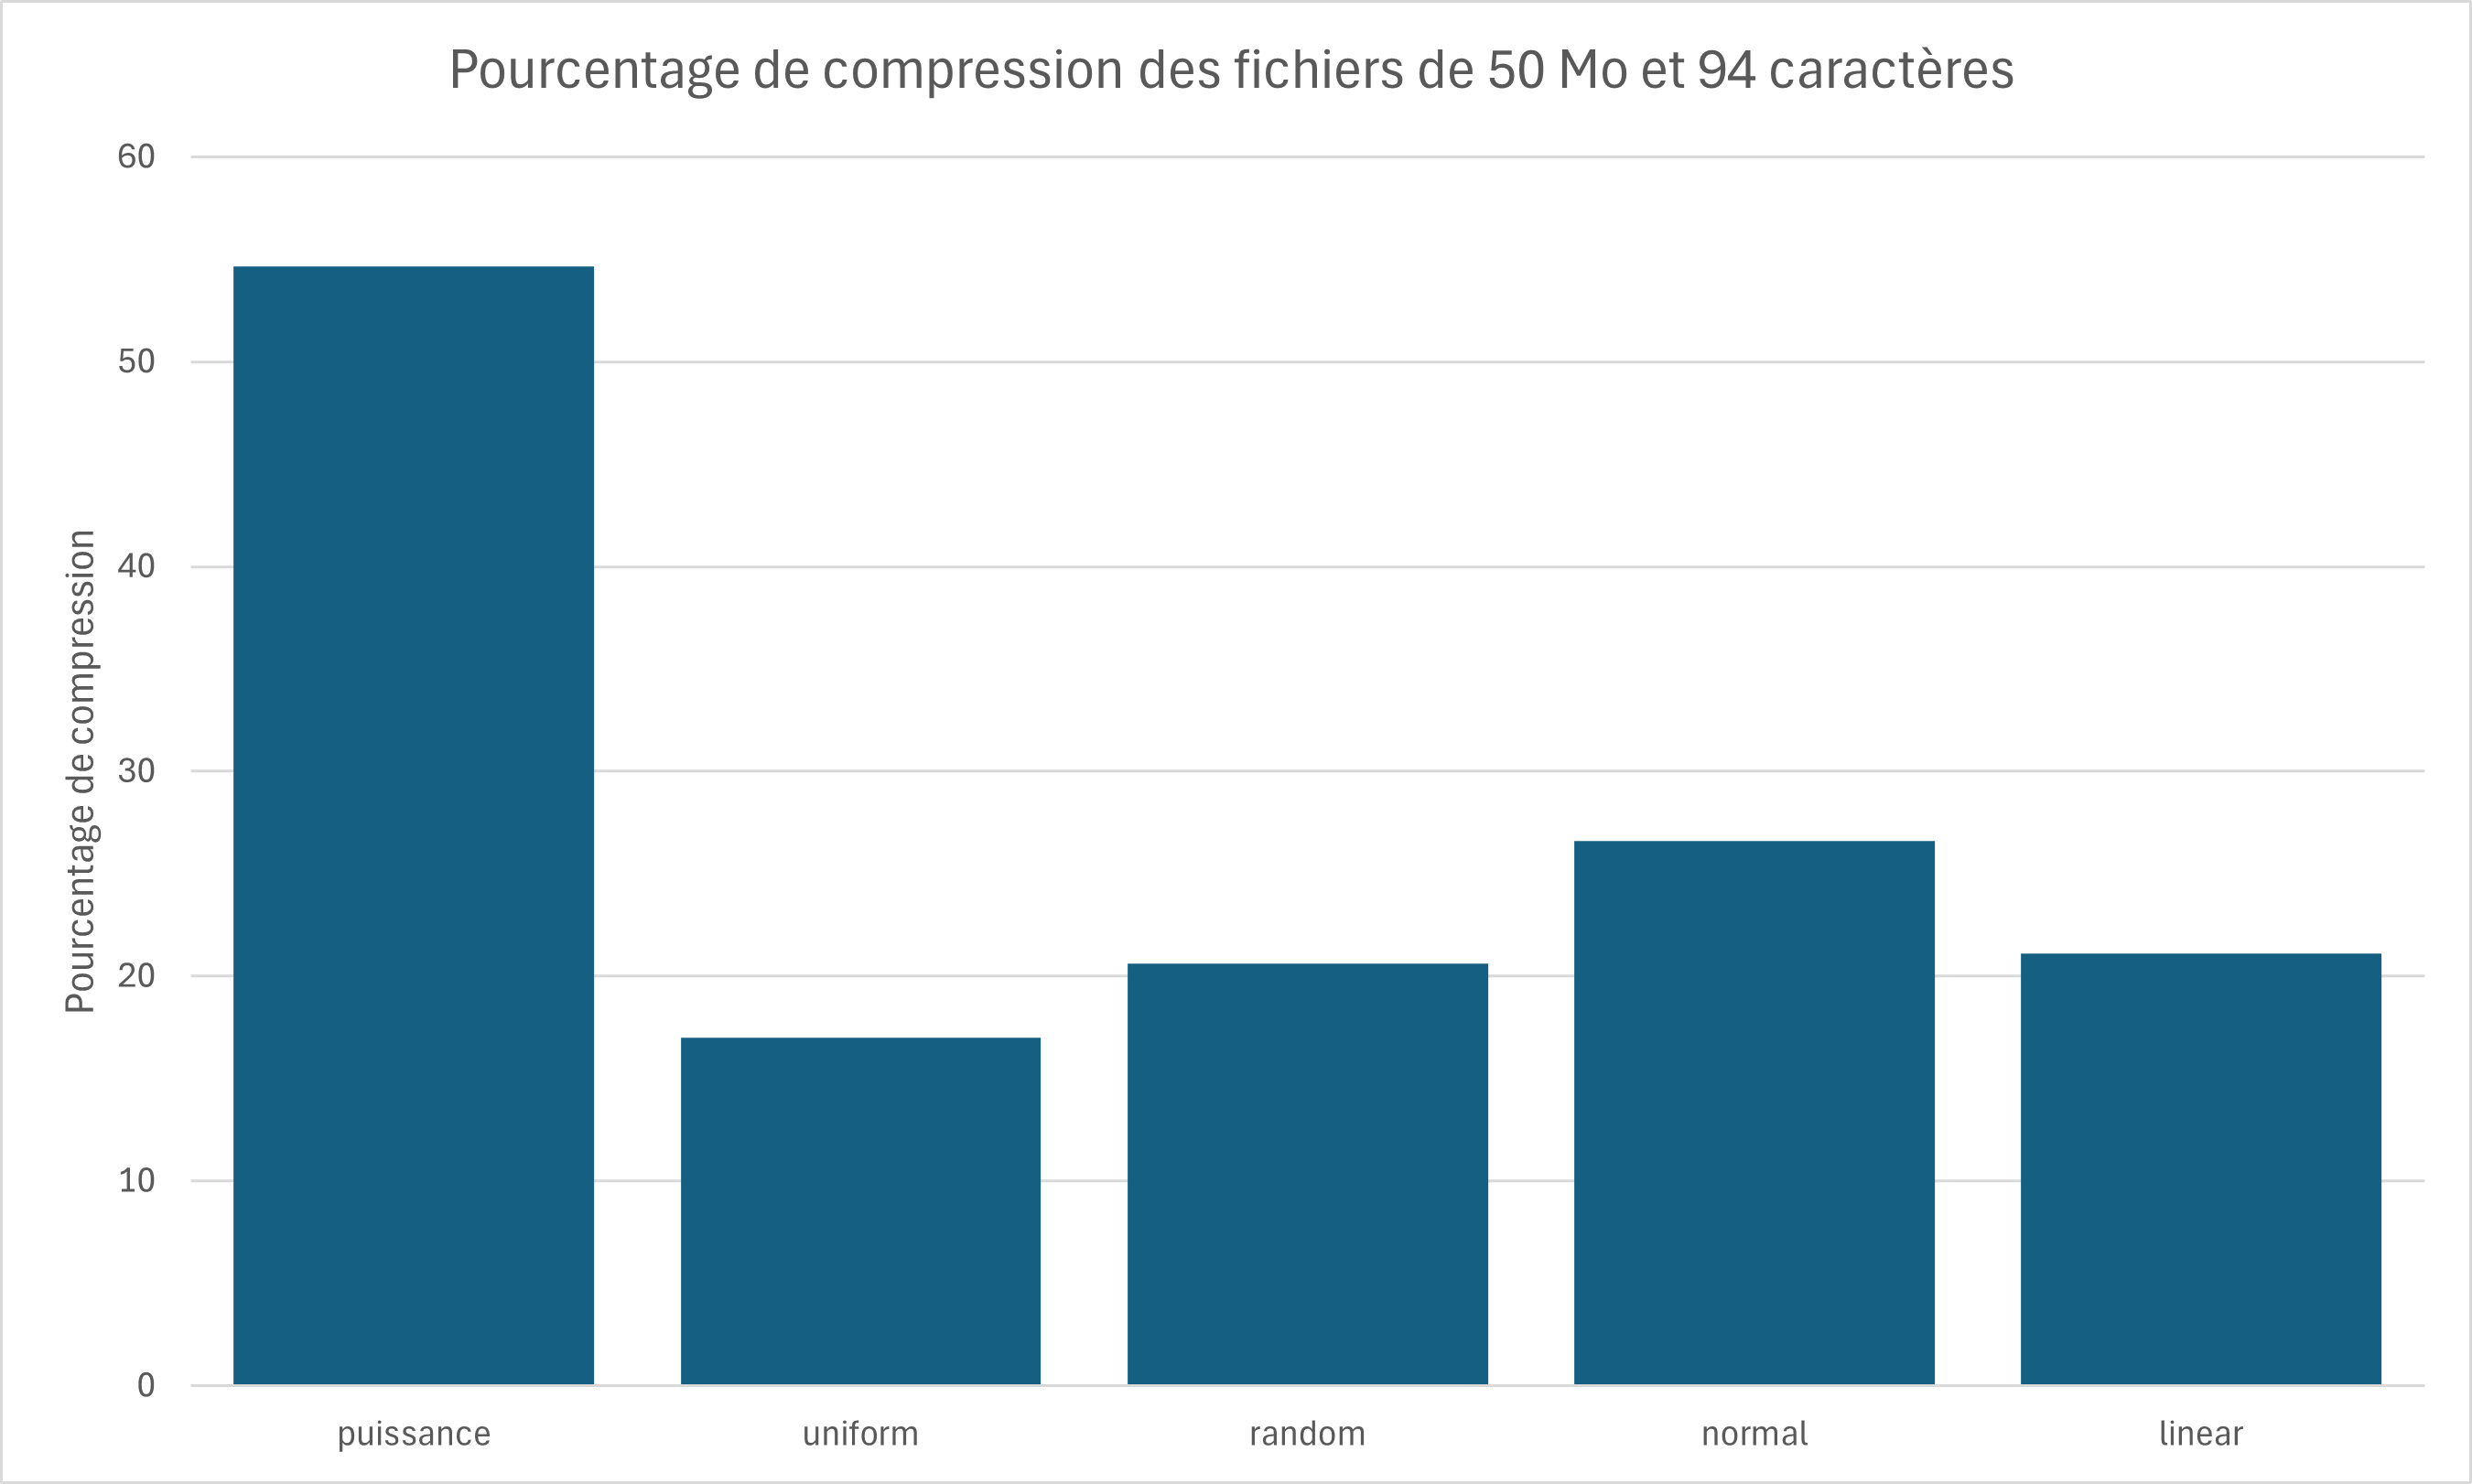
\includegraphics[width=\textwidth]{../assets/pourcentage-de-compression.png}
        \end{column}
    \end{columns}
\end{frame}

\subsection*{Evolution du taux de compression selon la taille de l'alphabet}
\begin{frame}{Evolution du taux de compression selon la taille de l'alphabet}
    \begin{columns}[T]
        \begin{column}{0.9\textwidth}
            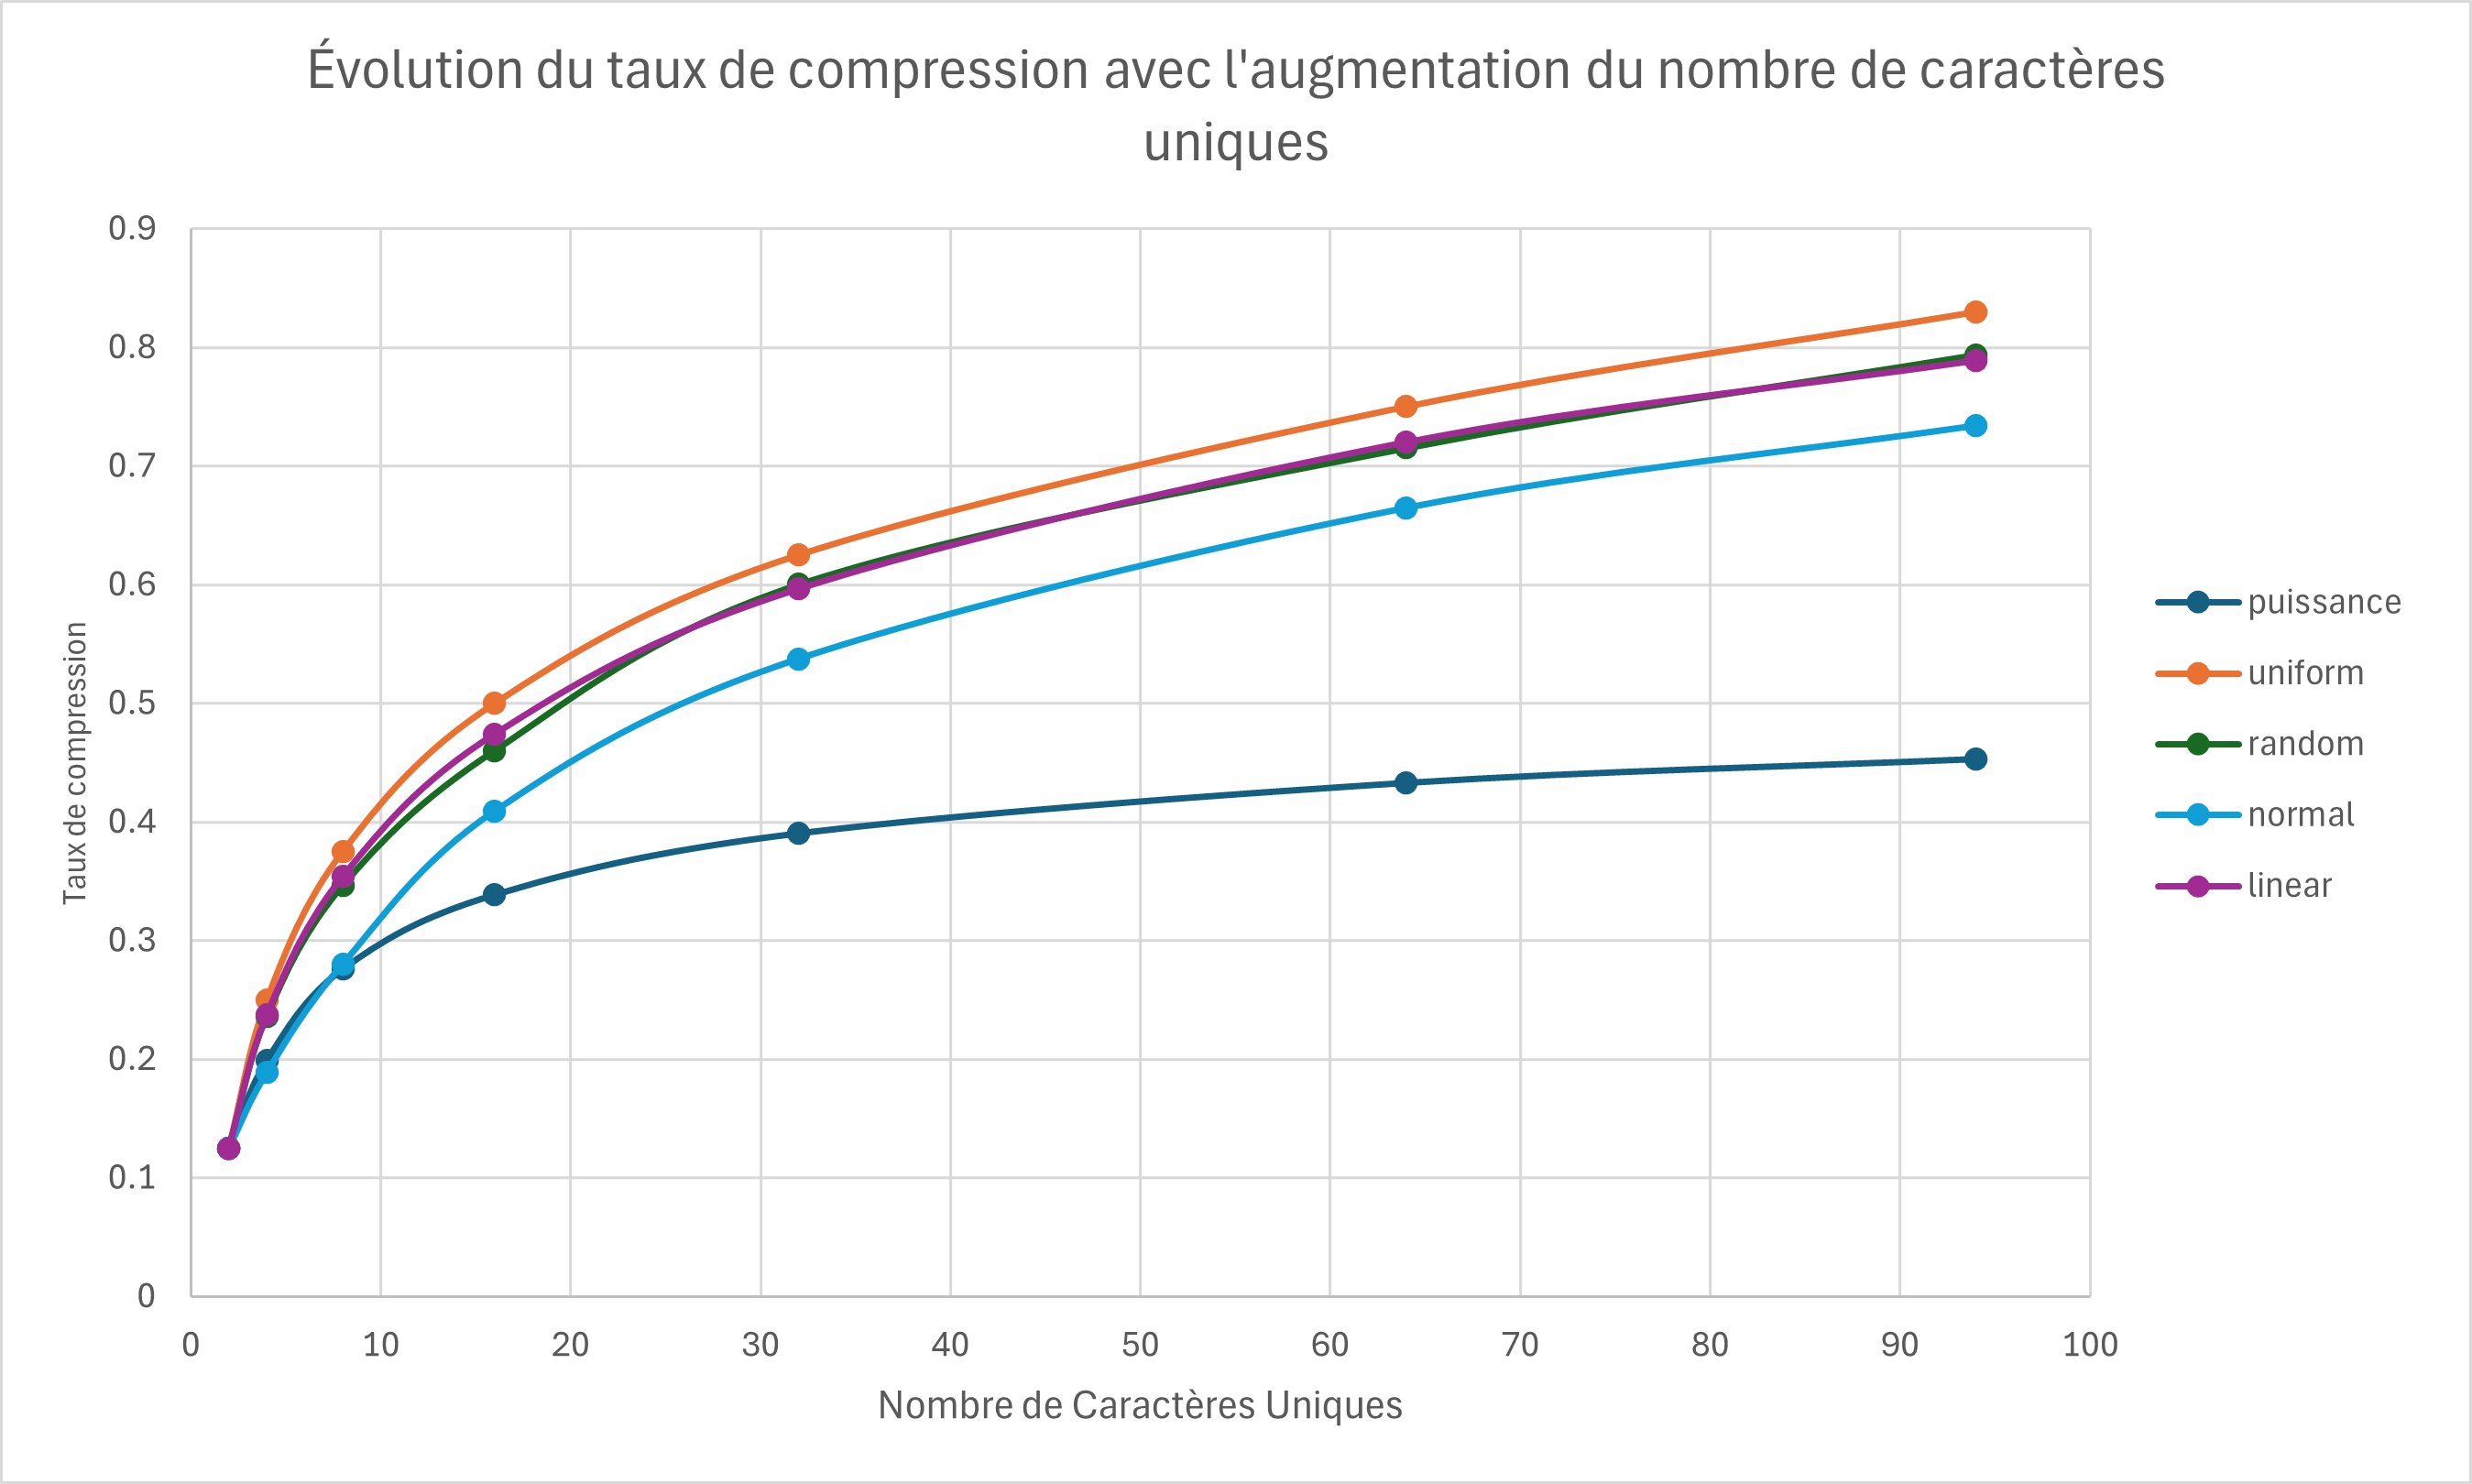
\includegraphics[width=\textwidth]{../assets/evolution-taux-de-compression-augmentation-unique-char.png}
        \end{column}
    \end{columns}
\end{frame}


\subsection*{Pourcentage de compression selon la taille du fichier original}
\begin{frame}{Analyse et interprétation}
    \begin{columns}[T]
        \begin{column}{0.9\textwidth}
            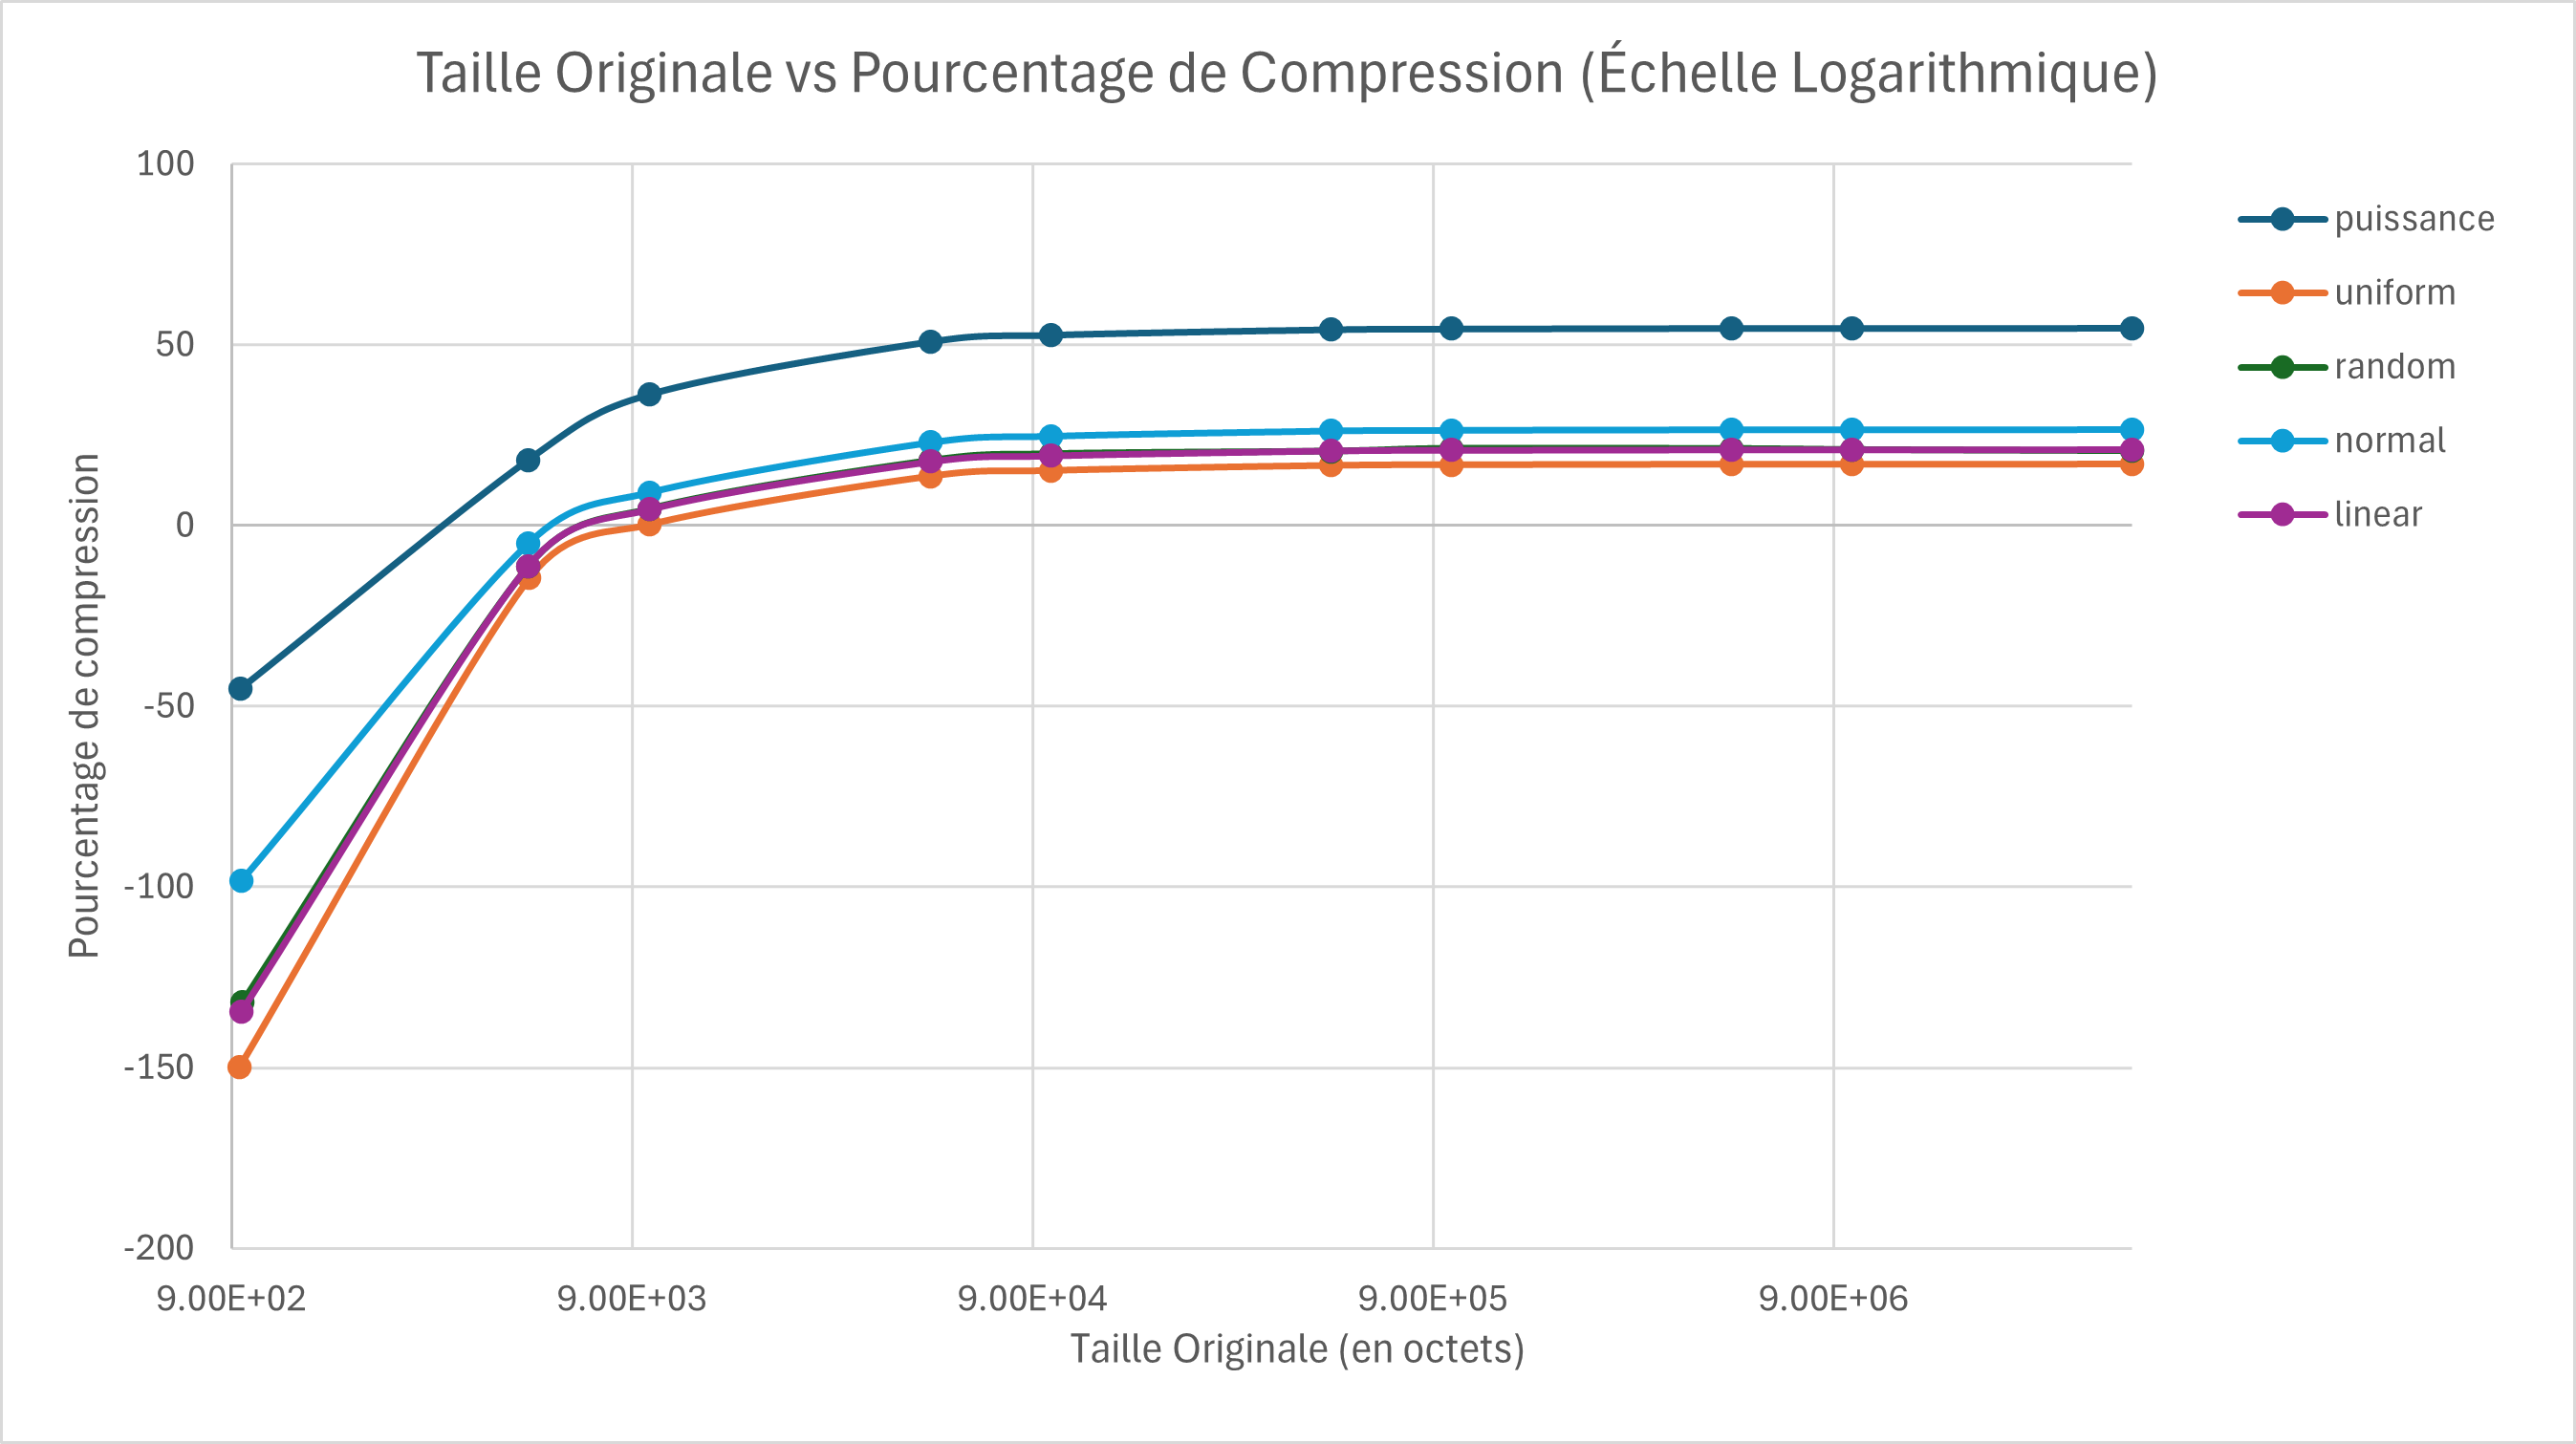
\includegraphics[width=\textwidth]{../assets/taille-original-vs-pourcentage-compression.png}
        \end{column}
    \end{columns}
\end{frame}

\section{Conclusion}

\begin{frame}{Conclusion}
    \begin{itemize}
        \item Une grande disparité des fréquences d'apparition des caractères favorise la compression
        \item La taille de l'alphabet influence le taux de compression
        \item Les taux de compression semblent converger vers une valeur limite pour des tailles de fichiers très grandes
    \end{itemize}
\end{frame}


\section{Demonstration}
\begin{frame}{Demonstration}
    \begin{itemize}
        \item Demonstration
    \end{itemize}
\end{frame}

\end{document}
